\documentclass[aspectratio=169,notheorems]{beamer}
\usetheme{default}
\usefonttheme{professionalfonts}
\setbeamersize{text margin left=8mm,text margin right=8mm}
\setbeamertemplate{navigation symbols}{}
\setbeamertemplate{footline}{%
  \leavevmode
  \hbox{\begin{beamercolorbox}[
    wd=\paperwidth,ht=2.5ex,dp=1.2ex,center
  ]{page number in head/foot}%
    \insertframenumber
  \end{beamercolorbox}}}
\setbeamertemplate{itemize item}{--}
\setbeamertemplate{itemize subitem}{--}

\usepackage{fontspec}
\setsansfont{Arial}
\setmainfont{Arial}
\XeTeXlinebreaklocale "en"
\usepackage{amsmath,amssymb,mathtools,booktabs,array}
\usepackage{microtype}
\newcolumntype{L}[1]{>{\raggedright\arraybackslash}p{#1}}

\definecolor{myblue}{RGB}{25,75,130}
\setbeamercolor{structure}{fg=myblue}
\setbeamercolor{frametitle}{fg=myblue}
\setbeamerfont{frametitle}{size=\large,series=\bfseries}
\setbeamertemplate{blocks}[rounded][shadow=false]
\setbeamercolor{block title}{fg=myblue,bg=myblue!12}
\setbeamercolor{block body}{bg=myblue!4}

\newcommand{\E}{\mathbb{E}}
\newcommand{\KL}{\mathrm{KL}}
\newcommand{\NLL}{\mathrm{NLL}}
\newcommand{\code}[1]{\texttt{#1}}
\newcommand{\take}[1]{%
  \par\vspace{0.35em}{\color{myblue}\hrule height 0.6pt}%
  \vspace{0.25em}\noindent\textbf{#1}\par}

% Editable diagrams and text code use the same restrained palette.
\usepackage{tikz,listings}
\usetikzlibrary{positioning,arrows.meta,calc}
\tikzset{
  flowbox/.style={draw=myblue!45,fill=myblue!4,rounded corners=2pt,
    inner sep=5pt,align=center,font=\footnotesize},
  flowarrow/.style={-{Stealth[length=2mm]},thick,myblue},
  family/.style={anchor=west,inner sep=2pt,font=\footnotesize}
}
\lstset{
  language=Python,
  basicstyle=\ttfamily\fontsize{8}{9.6}\selectfont,
  keywordstyle=\color{myblue}\bfseries,
  commentstyle=\color{black!65},
  stringstyle=\color{myblue},
  backgroundcolor=\color{myblue!4},
  frame=none,
  columns=fullflexible,
  keepspaces=true,
  showstringspaces=false,
  upquote=true,
  aboveskip=4pt,
  belowskip=4pt,
  xleftmargin=3pt,
  xrightmargin=3pt,
  breaklines=false
}


\title{DL Complexity: one interface, different measures}
\subtitle{Library architecture and BIC proof of concept}
\author{Alyabushev \and Dementiev \and Kurdyukov \and Chirkov}
\date{Proof of concept}
\hypersetup{
  pdftitle={DL Complexity: architecture and BIC proof of concept},
  pdfauthor={Alyabushev, Dementiev, Kurdyukov, Chirkov}
}

\begin{document}

\begin{frame}{DL Complexity: one interface, different measures}
\small
{\footnotesize Alyabushev, Dementiev, Kurdyukov, Chirkov
\hfill \code{dl\_complexity}}

\medskip
Evaluate model complexity through a common PyTorch-facing API,
while preserving the meaning of each measure.

\medskip
\centering
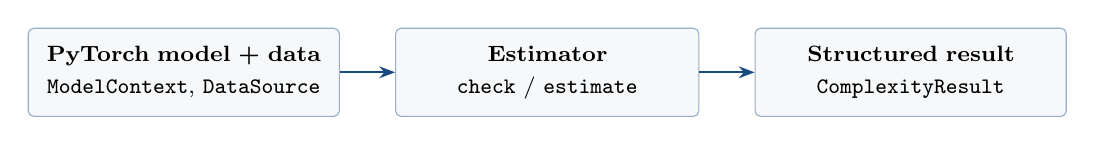
\begin{tikzpicture}
  \node[flowbox,text width=3.6cm,minimum height=1.12cm] (model)
    {\textbf{PyTorch model + data}\\[2pt]
     \code{ModelContext}, \code{DataSource}};
  \node[flowbox,text width=3.5cm,minimum height=1.12cm,right=7mm of model] (method)
    {\textbf{Estimator}\\[2pt]\code{check} / \code{estimate}};
  \node[flowbox,text width=3.6cm,minimum height=1.12cm,right=7mm of method] (result)
    {\textbf{Structured result}\\[2pt]\code{ComplexityResult}};
  \draw[flowarrow] (model) -- (method);
  \draw[flowarrow] (method) -- (result);
\end{tikzpicture}
\par
\medskip
\begin{columns}[T,onlytextwidth]
  \begin{column}{.315\textwidth}
    \begin{block}{Information criteria}
      \small AIC, BIC, WAIC\\[3pt]
      Fit and complexity penalties\\
      \code{native\_ic}
    \end{block}
  \end{column}
  \begin{column}{.315\textwidth}
    \begin{block}{Code lengths}
      \small Two-part and prequential MDL\\[3pt]
      Description of model/data\\
      \code{nats} or \code{bits}
    \end{block}
  \end{column}
  \begin{column}{.315\textwidth}
    \begin{block}{Risk bounds}
      \small Compression-based bounds\\[3pt]
      Generalization guarantees\\
      Risk scale, under assumptions
    \end{block}
  \end{column}
\end{columns}
\raggedright
\medskip
\take{One calling convention does not imply one scale or a universal ranking.}
\end{frame}

\begin{frame}{Core objects and data flow}
\small
\centering
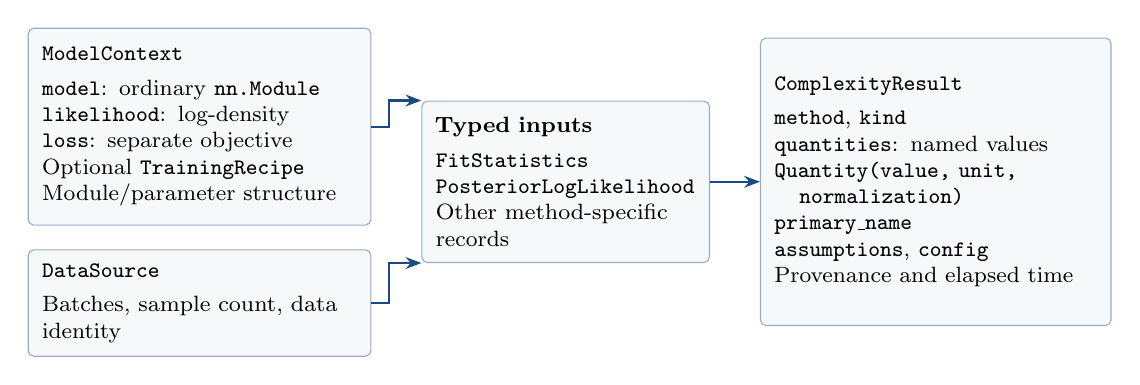
\begin{tikzpicture}
  \node[flowbox,align=left,text width=4.0cm,minimum height=2.5cm] (context) at (0,0)
    {\textbf{\code{ModelContext}}\\[3pt]
     \code{model}: ordinary \code{nn.Module}\\
     \code{likelihood}: log-density\\
     \code{loss}: separate objective\\
     Optional \code{TrainingRecipe}\\
     Module/parameter structure};
  \node[flowbox,align=left,text width=4.0cm,minimum height=1.1cm,below=3mm of context] (data)
    {\textbf{\code{DataSource}}\\[3pt]
     Batches, sample count, data identity};
  \node[flowbox,align=left,text width=3.3cm,minimum height=2.05cm] (inputs) at (4.65,-.7)
    {\textbf{Typed inputs}\\[3pt]
     \code{FitStatistics}\\
     {\fontsize{8}{9.6}\selectfont\code{PosteriorLogLikelihood}}\\
     Other method-specific records};
  \node[flowbox,align=left,text width=4.1cm,minimum height=3.65cm] (result) at (9.35,-.7)
    {\textbf{\code{ComplexityResult}}\\[3pt]
     \code{method}, \code{kind}\\
     \code{quantities}: named values\\
     \code{Quantity(value, unit,}\\
     \hspace*{9pt}\code{normalization)}\\
     \code{primary\_name}\\
     \code{assumptions}, \code{config}\\
     Provenance and elapsed time};
  \draw[flowarrow] (context.east) -- ++(.22,0) |- (inputs.north west);
  \draw[flowarrow] (data.east) -- ++(.22,0) |- (inputs.south west);
  \draw[flowarrow] (inputs.east) -- (result.west);
\end{tikzpicture}
\par
\smallskip
\raggedright
{\footnotesize Direct preparation is method-specific; posterior samples are supplied explicitly.\\
Prepared records can also be passed without a model.}
\raggedright
\medskip
\begin{itemize}\setlength{\itemsep}{.2em}
  \item A loss is not automatically a negative log-likelihood; the relation must be explicit.
  \item Training is explicit. A recipe stores instructions, not an implicit call to fit.
\end{itemize}
\end{frame}

\begin{frame}{Base classes and extension points}
\small
\begin{columns}[T,onlytextwidth]
\begin{column}{.49\textwidth}
\textbf{Estimator inheritance}
\smallskip

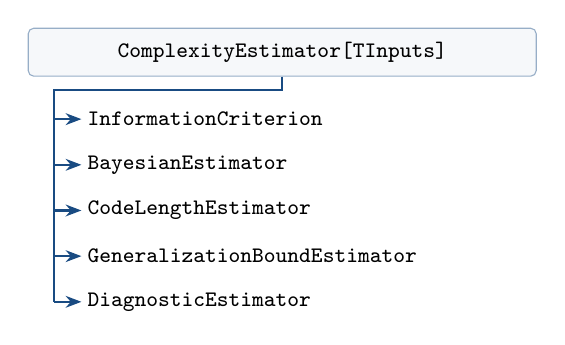
\begin{tikzpicture}
  \node[flowbox,text width=6.1cm,minimum height=.56cm] (base)
    {\code{ComplexityEstimator[TInputs]}};
  \node[family] (ic) at (-2.55,-.85) {\code{InformationCriterion}};
  \node[family] (bayes) at (-2.55,-1.43) {\code{BayesianEstimator}};
  \node[family] (code) at (-2.55,-2.01) {\code{CodeLengthEstimator}};
  \node[family] (bound) at (-2.55,-2.59) {\code{GeneralizationBoundEstimator}};
  \node[family] (diag) at (-2.55,-3.17) {\code{DiagnosticEstimator}};
  \coordinate (trunk) at (-2.9,-.5);
  \draw[myblue,thick] (base.south) -- (0,-.48) -| (trunk) -- (-2.9,-3.17);
  \foreach \child in {ic,bayes,code,bound,diag}
    \draw[flowarrow] (-2.9,0 |- \child.west) -- (\child.west);
\end{tikzpicture}
{\scriptsize Branches point from a base to its subclasses.}
\end{column}
\begin{column}{.48\textwidth}
\begin{block}{Public protocol}
\footnotesize
\code{check(...)} $\rightarrow$ \code{RequirementReport}\\[3pt]
\code{estimate(...)} $\rightarrow$ \code{ComplexityResult}\\[3pt]
Pass \code{context} + \code{data}, or \code{inputs}.
\end{block}
\begin{block}{Implementing a method}
\footnotesize
\begin{itemize}\setlength{\itemsep}{.15em}
  \item Declare \code{input\_type}.
  \item Implement \code{\_estimate(inputs)}.
  \item Optional checks: \code{\_check\_inputs}.
  \item For a direct route, add \code{\_check\_context} and \code{\_prepare\_context}.
\end{itemize}
\end{block}
\end{column}
\end{columns}
\smallskip
\begin{block}{Separate interfaces, not estimator subclasses}
\code{ModelTransform.apply(model)}
\hfill
\code{ModelCodec.encode(model)} / \code{decode(artifact)}
\end{block}
\end{frame}

\begin{frame}[fragile]{User workflow: check, estimate, reuse}
\small
\begin{columns}[T,onlytextwidth]
\begin{column}{.605\textwidth}
\textbf{Direct route: model + observations}
\begin{lstlisting}
x = torch.ones(4, 1, dtype=torch.float64)
y = torch.tensor([1., 2., 4., 5.],
                 dtype=torch.float64)[:, None]
model = nn.Linear(1, 1, bias=False,
                  dtype=torch.float64)
with torch.no_grad():
    model.weight.fill_(3.)  # analytic MLE
context = ModelContext(model,
    likelihood=GaussianLikelihood(sigma=1.))
data = DataSource.from_tensors(x, y)
bic = BIC()
report = bic.check(context, data=data)
if report.ready:
    result = bic.estimate(context, data=data)
\end{lstlisting}
{\scriptsize Imports and the runnable example are in \code{presentation/README.md}.}
\end{column}
\begin{column}{.37\textwidth}
\textbf{Prepared route}
\begin{lstlisting}
stats = FitStatistics(
    log_likelihood=ll,
    k=1, n=4)
prepared = bic.estimate(
    inputs=stats)
\end{lstlisting}
{\footnotesize \code{ll}: total natural log-likelihood at the fitted parameters.
Reuse the same statistics for AIC/BIC/HQIC without another model pass.}
\begin{block}{\code{ComplexitySuite}}
\footnotesize Runs named estimators and returns an \code{EvaluationOutcome} per method.
No implicit fitting, shared cache or cross-measure ranking.
\end{block}
\end{column}
\end{columns}
\smallskip
\take{Fit explicitly; \code{check} inspects readiness; \code{estimate} computes the measure.}
\end{frame}

\begin{frame}[fragile]{BIC inside the architecture}
\centering
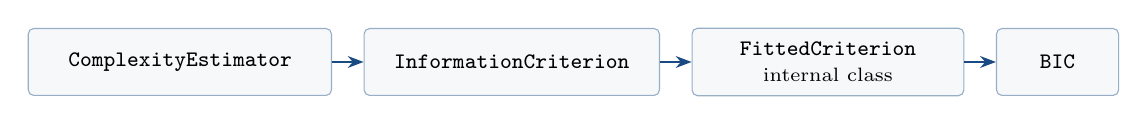
\begin{tikzpicture}
  \node[flowbox,text width=3.5cm,minimum height=.85cm] (base)
    {\code{ComplexityEstimator}};
  \node[flowbox,text width=3.4cm,minimum height=.85cm,right=4mm of base] (ic)
    {\code{InformationCriterion}};
  \node[flowbox,text width=3.1cm,minimum height=.85cm,right=4mm of ic] (fit)
    {\code{FittedCriterion}\\{\scriptsize internal class}};
  \node[flowbox,text width=1.2cm,minimum height=.85cm,right=4mm of fit] (bic)
    {\code{BIC}};
  \draw[flowarrow] (base) -- (ic);
  \draw[flowarrow] (ic) -- (fit);
  \draw[flowarrow] (fit) -- (bic);
\end{tikzpicture}
\par
\raggedright
\medskip
\begin{columns}[T,onlytextwidth]
\begin{column}{.50\textwidth}
\begin{block}{Method-specific calculation}
\[
  \mathrm{BIC} =
  \underbrace{-2\log L(\hat\theta)}_{\text{deviance}}
  + \underbrace{k\log n}_{\text{penalty}}
\]
\begin{lstlisting}
ll, k, n = self._statistics(inputs)
deviance = -2 * ll
penalty = ll.new_tensor(k * math.log(n))
\end{lstlisting}
{\scriptsize Exact excerpt: \code{criteria/bic.py}, \code{BIC.\_estimate}.}
\end{block}
\end{column}
\begin{column}{.47\textwidth}
\begin{block}{Shared preparation}
\small
\code{FittedCriterion} obtains \code{FitStatistics}: total log-likelihood, parameter count and sample count.
\end{block}
\begin{block}{Standard output}
\small
\code{BIC} returns \code{bic}, \code{deviance}, \code{penalty} in \code{quantities}.\\[3pt]
Unit: \code{native\_ic}; normalization: \code{total}.
\end{block}
\end{column}
\end{columns}
\smallskip
{\footnotesize Formula cost: $O(1)$ after preparation; the direct route also evaluates the model.
BIC assumes a regular finite-dimensional MLE setting.}
\small
\take{\code{check().ready} does not establish MLE optimality or BIC's asymptotic assumptions.}
\end{frame}

\begin{frame}{Proof of concept: analytic reference vs library}
\small
$y=(1,2,4,5)$,\quad $y_i\sim\mathcal{N}(\mu,1)$,\quad
$\hat\mu=\bar y=3$,\quad $n=4$,\quad $k=1$.
\[
  \sum_i(y_i-\hat\mu)^2=10,\qquad
  \ell(\hat\mu)=-\frac{4}{2}\log(2\pi)-\frac{10}{2}.
\]
\centering
{\footnotesize
\setlength{\tabcolsep}{7pt}
\renewcommand{\arraystretch}{1.22}
\begin{tabular}{@{}lrrr@{}}
\toprule
\textbf{Quantity} & \textbf{Analytic reference}
 & \textbf{Model + data} & \textbf{FitStatistics}\\
\midrule
Deviance & 17.35150826563738 & 17.35150826563738 & 17.35150826563738\\
Penalty  & 1.38629436111989 & 1.38629436111989 & 1.38629436111989\\
\textbf{BIC} & \textbf{18.73780262675727} & \textbf{18.73780262675727} & \textbf{18.73780262675727}\\
\bottomrule
\end{tabular}
}
\par
\smallskip
\begin{block}{Standard result: \code{native\_ic}, \code{total}}
\small Both public routes agree with the independent formula to $10^{-12}$.
\end{block}
\raggedright
\footnotesize
\begin{itemize}\setlength{\itemsep}{.15em}
  \item Five known-variance Gaussian cases pass the selected analytical tests.
  \item This is an integration PoC, not a full benchmark or a proof for arbitrary neural networks.
\end{itemize}
{\scriptsize Source: \code{tests/test\_analytical\_criteria.py}, \code{test\_gaussian\_mean\_mle\_known\_variance}.}
\take{BIC uses shared preparation and returns the standard structured result.}
\end{frame}

\end{document}
